\documentclass{beamer}

%----------------------------------------------------------------------------------------
%   PACKAGES AND THEMES
%----------------------------------------------------------------------------------------
\usepackage[utf8]{inputenc}
\usepackage[T1]{fontenc}
\usepackage{graphicx}
\usepackage[spanish]{babel}
\usepackage{textpos} % Para posicionar el logo en todas las diapositivas
\usepackage{tikz}
\usepackage[round]{natbib}
\bibliographystyle{abbrvnat}
\usetikzlibrary{fadings}
\usetikzlibrary{patterns}
\usetikzlibrary{shadows.blur}
\usetikzlibrary{shapes}
\usetheme{Darmstadt}

\setbeamertemplate{navigation symbols}{}
\setbeamertemplate{footline}[frame number]

%----------------------------------------------------------------------------------------
%   TITLE PAGE
%----------------------------------------------------------------------------------------
\title{Estudio del \textit{trade-off} en decisiones financieras sostenibles}
\subtitle{Defensa Tesis Ingeniería Civil Industrial}
\author{Vicente Tejero}
\institute[Universidad de los Andes]
{
    Universidad de los Andes \\
    \medskip
    \textit{Profesor guía: Sebastián Cea}
}
\date{\today}

%----------------------------------------------------------------------------------------
%   POSITION THE LOGO
%----------------------------------------------------------------------------------------
\addtobeamertemplate{frametitle}{}{%
\begin{textblock*}{100mm}(-0.05\textwidth,6.2cm) % Ajusta las coordenadas para mover el logo a la esquina inferior izquierda
\includegraphics[width=1cm]{log.png}
\end{textblock*}}


\begin{document}

\begin{frame}
    \titlepage
\end{frame}

\begin{frame}
    \tableofcontents
\end{frame}

%----------------------------------------------------------------------------------------
%   PRESENTATION SLIDES
%----------------------------------------------------------------------------------------
\section{Introducción}


\begin{frame}
    \frametitle{Objetivos y Metodología}
    % ESPECIFICAR CÖMO SE ABORDA o QUÉ PARTE SE ABORDA
    \begin{itemize}
        \item \textbf{Objetivos:} Testear la coherencia en las decisiones de inversión con el grado de atención de los inversores a métricas ASG, tomando en cuenta que dichas métricas tienen características de bien público.
        \item \textbf{Metodología:} Uso de un marco teórico y experimental de preferencias y valoración contingente junto con el monitoreo de la atención de los participantes mediante:
        \begin{itemize}
            \item Dilatación pupilar 
            \item \emph{Cognitive reflection test}
            \item Autoreporte (preferencias por información o valor revelado)
        \end{itemize}
    \end{itemize}
\end{frame}

\begin{frame}
    \frametitle{Contribución Académica}

     Este trabajo se diferencia por integrar métricas biométricas para evaluar directamente la carga cognitiva y la atención, un enfoque prácticamente no explorado en estudios anteriores sobre finanzas sostenibles.

\begin{itemize}
    \item Teoría: 
    \begin{itemize}
        \item Aplicación de un marco de agregación de preferencias sobre criterios sociales \cite{decancq_chapter_2015,burone_measuring_2023}
        \item Inclusión de valorización contingente \cite{cooper_one-and-one-half-bound_2002}
    \end{itemize}
    \item Experimento:
    \begin{itemize}
        \item Configuración de valorización de un bien público \cite{chan_cost-effective_2024}
        \item Medición de atención
        \begin{itemize}
            \item Cognitive reflection test \cite{frederick_cognitive_2005,sirota_effect_2018}
        \item Monitoreo de dilatación pupilar \cite{geller_gazer_2020}
        \end{itemize}        
    \end{itemize}
\end{itemize}
\end{frame}


\section{Marco Teórico}


\begin{frame}
    \frametitle{Costo de Cambio/Disposición a Pagar}
    \begin{itemize}
        \item Costo de cambio puede ser tratado cómo la disposición a pagar. Ejemplo, si un inversionista acepta perder un 2\% de
        rentabilidad monetaria por aumentar su retorno sostenible significa que el individuo está dispuesto
        a pagar por lo menos con un 2\% de rentabilidad pecuniaria.
    \end{itemize}
    \begin{figure}
        \centering
        


\tikzset{every picture/.style={line width=0.75pt}} %set default line width to 0.75pt        

\begin{tikzpicture}[x=0.4pt,y=0.4pt,yscale=-1,xscale=1]
%uncomment if require: \path (0,310); %set diagram left start at 0, and has height of 310

%Shape: Axis 2D [id:dp13395617326038134] 
\draw  (63.29,240.77) -- (317,240.77)(88.66,15) -- (88.66,265.86) (310,235.77) -- (317,240.77) -- (310,245.77) (83.66,22) -- (88.66,15) -- (93.66,22)  ;
%Curve Lines [id:da4183460986445604] 
\draw  [dash pattern={on 0.84pt off 2.51pt}]  (99.5,50.2) .. controls (109.6,152.2) and (196.4,177.4) .. (289.5,175.2) ;
%Straight Lines [id:da5546289245074529] 
\draw  [dash pattern={on 4.5pt off 4.5pt}]  (249.8,181.2) -- (249.8,241.2) ;
%Straight Lines [id:da17230577782004053] 
\draw  [dash pattern={on 4.5pt off 4.5pt}]  (101.4,75.6) -- (102.6,242.6) ;
%Straight Lines [id:da15960024650457827] 
\draw  [dash pattern={on 4.5pt off 4.5pt}]  (247,174) -- (88.2,174.2) ;
%Straight Lines [id:da8852960475718443] 
\draw  [dash pattern={on 4.5pt off 4.5pt}]  (96.4,66) -- (87.4,66.2) ;
%Straight Lines [id:da6895250979600871] 
\draw [color={rgb, 255:red, 208; green, 2; blue, 27 }  ,draw opacity=1 ]   (81.2,67) -- (81,172.6) ;
\draw [shift={(81,174.6)}, rotate = 270.11] [color={rgb, 255:red, 208; green, 2; blue, 27 }  ,draw opacity=1 ][line width=0.75]    (10.93,-3.29) .. controls (6.95,-1.4) and (3.31,-0.3) .. (0,0) .. controls (3.31,0.3) and (6.95,1.4) .. (10.93,3.29)   ;
%Straight Lines [id:da11332460849697212] 
\draw [color={rgb, 255:red, 65; green, 117; blue, 5 }  ,draw opacity=1 ]   (102.2,245.8) -- (247.4,246.59) ;
\draw [shift={(249.4,246.6)}, rotate = 180.31] [color={rgb, 255:red, 65; green, 117; blue, 5 }  ,draw opacity=1 ][line width=0.75]    (10.93,-3.29) .. controls (6.95,-1.4) and (3.31,-0.3) .. (0,0) .. controls (3.31,0.3) and (6.95,1.4) .. (10.93,3.29)   ;

% Text Node
\draw (49.9,11.2) node [anchor=north west][inner sep=0.75pt]    {$x{^{\ }}^{\$}$};
% Text Node
\draw (292.5,250.5) node [anchor=north west][inner sep=0.75pt]    {$x{^{\ }}^{ASG}$};
% Text Node
\draw (105.3,43) node [anchor=north west][inner sep=0.75pt]    {$\ell _{j}$};

% Text Node
\draw (240.8,171.4) node [anchor=north west][inner sep=0.75pt]  [font=\fontsize{3em}{3.6em}\selectfont,color={rgb, 255:red, 208; green, 2; blue, 27 }  ,opacity=1 ] [align=left] {.};
% Text Node
\draw (94.6,53) node [anchor=north west][inner sep=0.75pt]  [font=\fontsize{3em}{3.6em}\selectfont,color={rgb, 255:red, 74; green, 144; blue, 226 }  ,opacity=1 ] [align=left] {.};

\draw (250.5,145.4) node [anchor=north west][inner sep=0.75pt]    {$\ell '_{j}$};

% Text Node
\draw (20,111.6) node [anchor=north west][inner sep=0.75pt]  [font=\scriptsize,color={rgb, 255:red, 208; green, 2; blue, 27 }  ,opacity=1 ] [align=left] {\mbox{-}2\% $\displaystyle \$$};
% Text Node
\draw (122,247.2) node [anchor=north west][inner sep=0.75pt]  [font=\scriptsize,color={rgb, 255:red, 65; green, 117; blue, 5 }  ,opacity=1 ] [align=left] {+2\% $\displaystyle ASG$};


\end{tikzpicture}
        \caption{Ejemplo disposición a pagar}
    \end{figure}
\end{frame}

\begin{frame}
\frametitle{Valorización Contingente}
Se realizó una valorización contingente siguiendo la metodología de \cite{chalmer_economic_2021}, el cual formula la siguiente pregunta: `¿Estas dispuesto a aceptar una tasa de rendimiento más baja a cambio de un beneficio social o ambiental?'
    \begin{figure}
        \centering
        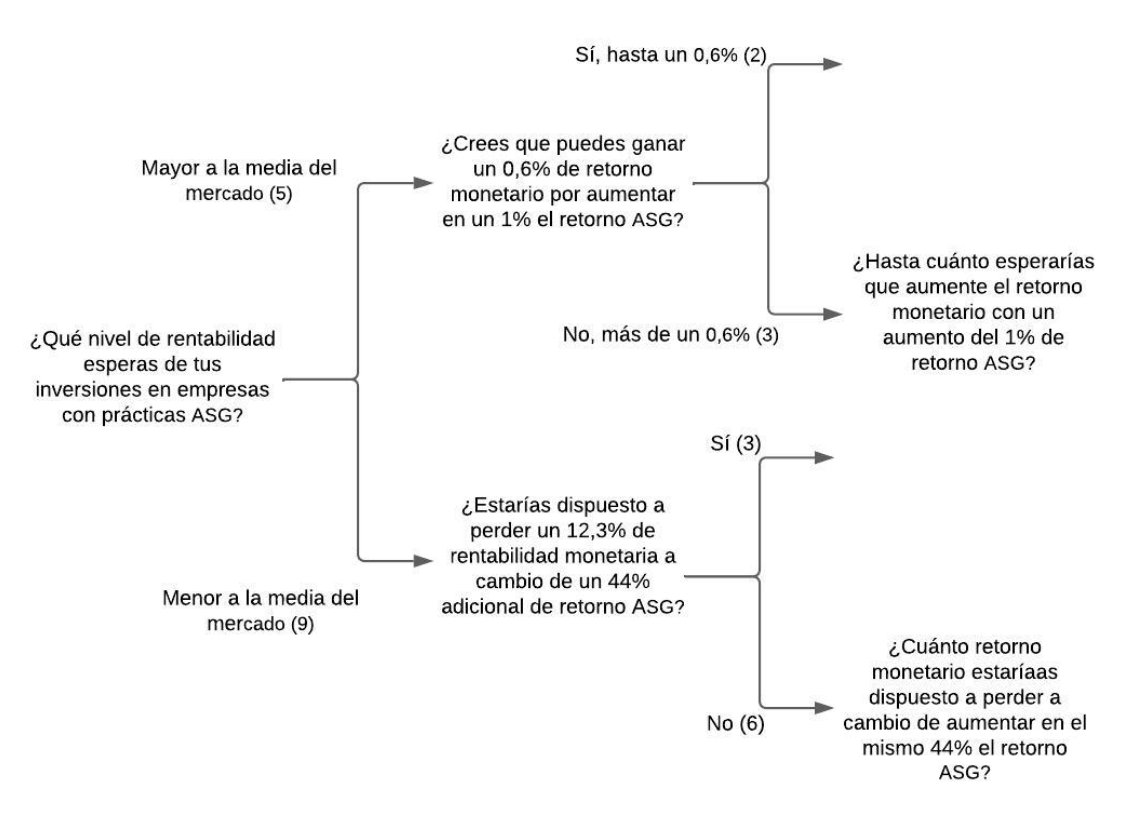
\includegraphics[width=0.55\linewidth]{DiagramaValorizacionContingente.png}
        \caption{Diagrama Valorización Contingente}
    \end{figure}
\end{frame}




\begin{frame}

\begin{minipage}{0.45\textwidth}
    Cada punto negro representa el ASG subjetivo determinado por cada proveedor, identificado como $ASG_0$, $ASG_1$ y $ASG_2$, con el mismo nivel de rentabilidad ($\$_0$), mientras que el punto sin relleno representa el ASG objetivo, que podría considerarse como una ponderación de todos los proveedores.
\end{minipage}
\hfill
\begin{minipage}{0.5\textwidth}
    \begin{figure}
        \centering
        \tikzset{every picture/.style={line width=0.75pt}}
        \begin{tikzpicture}[x=0.45pt,y=0.45pt,yscale=-1,xscale=1]
            %uncomment if require: \path (0,403); %set diagram left start at 0, and has height of 403

            %Shape: Axis 2D [id:dp44817206223413786] 
            \draw [line width=0.75]  (87.7,351.95) -- (398.35,351.95)(118.77,75.51) -- (118.77,382.66) (391.35,346.95) -- (398.35,351.95) -- (391.35,356.95) (113.77,82.51) -- (118.77,75.51) -- (123.77,82.51)  ;
            %Straight Lines [id:da2635177468922987] 
            \draw    (113.55,127.43) -- (123.59,127.43) ;
            %Straight Lines [id:da12445618867563701] 
            \draw    (113.55,286.11) -- (123.59,286.11) ;
            %Straight Lines [id:da10735169417411794] 
            \draw    (113.06,207.75) -- (123.1,207.75) ;
            %Straight Lines [id:da3662912069748514] 
            \draw    (185.54,346.84) -- (185.3,356.14) ;
            %Straight Lines [id:da23171967171945718] 
            \draw    (256.07,347.33) -- (255.83,356.63) ;
            %Straight Lines [id:da14001372701656223] 
            \draw    (324.15,347.33) -- (323.9,356.63) ;
            %Straight Lines [id:da36090377200564694] 
            \draw [color={rgb, 255:red, 0; green, 0; blue, 0 }  ,draw opacity=0.13 ]   (113.55,127.43) -- (387.33,128.9) ;
            %Straight Lines [id:da7470745746754253] 
            \draw [color={rgb, 255:red, 0; green, 0; blue, 0 }  ,draw opacity=0.13 ]   (113.06,207.75) -- (387.33,208.48) ;
            %Straight Lines [id:da0014179812149808235] 
            \draw [color={rgb, 255:red, 0; green, 0; blue, 0 }  ,draw opacity=0.13 ]   (113.55,286.11) -- (388.55,286.84) ;
            %Straight Lines [id:da21484429021982154] 
            \draw [color={rgb, 255:red, 0; green, 0; blue, 0 }  ,draw opacity=0.14 ][fill={rgb, 255:red, 128; green, 128; blue, 128 }  ,fill opacity=0.36 ]   (185.3,88.49) -- (184.89,121.3) -- (185.3,356.14) ;
            %Straight Lines [id:da4031975643793815] 
            \draw [color={rgb, 255:red, 0; green, 0; blue, 0 }  ,draw opacity=0.14 ][fill={rgb, 255:red, 128; green, 128; blue, 128 }  ,fill opacity=0.36 ]   (256.56,88.98) -- (255.83,356.63) ;
            %Straight Lines [id:da1102018710260293] 
            \draw [color={rgb, 255:red, 0; green, 0; blue, 0 }  ,draw opacity=0.14 ][fill={rgb, 255:red, 128; green, 128; blue, 128 }  ,fill opacity=0.36 ]   (323.66,89.71) -- (323.9,356.63) ;
            %Shape: Ellipse [id:dp211780464841973] 
            \draw  [color={rgb, 255:red, 0; green, 0; blue, 0 }  ,draw opacity=1 ][fill={rgb, 255:red, 0; green, 0; blue, 0 }  ,fill opacity=1 ] (251.94,127.91) .. controls (251.94,125.34) and (254.02,123.26) .. (256.59,123.26) .. controls (259.16,123.26) and (261.24,125.34) .. (261.24,127.91) .. controls (261.24,130.48) and (259.16,132.56) .. (256.59,132.56) .. controls (254.02,132.56) and (251.94,130.48) .. (251.94,127.91) -- cycle ;
            %Straight Lines [id:da2776117172154504] 
            \draw [color={rgb, 255:red, 0; green, 0; blue, 0 }  ,draw opacity=0.14 ][fill={rgb, 255:red, 128; green, 128; blue, 128 }  ,fill opacity=0.36 ]   (387.33,90.94) -- (387.57,354.19) ;
            %Shape: Ellipse [id:dp2845497497287104] 
            \draw  [color={rgb, 255:red, 0; green, 0; blue, 0 }  ,draw opacity=1 ][fill={rgb, 255:red, 0; green, 0; blue, 0 }  ,fill opacity=1 ] (180.24,127.45) .. controls (180.24,124.88) and (182.32,122.8) .. (184.89,122.8) .. controls (187.46,122.8) and (189.55,124.88) .. (189.55,127.45) .. controls (189.55,130.02) and (187.46,132.11) .. (184.89,132.11) .. controls (182.32,132.11) and (180.24,130.02) .. (180.24,127.45) -- cycle ;
            %Shape: Ellipse [id:dp7185708332857657] 
            \draw  [color={rgb, 255:red, 0; green, 0; blue, 0 }  ,draw opacity=1 ][fill={rgb, 255:red, 0; green, 0; blue, 0 }  ,fill opacity=1 ] (318.82,128.16) .. controls (318.82,125.59) and (320.9,123.51) .. (323.47,123.51) .. controls (326.04,123.51) and (328.12,125.59) .. (328.12,128.16) .. controls (328.12,130.73) and (326.04,132.81) .. (323.47,132.81) .. controls (320.9,132.81) and (318.82,130.73) .. (318.82,128.16) -- cycle ;
            %Shape: Ellipse [id:dp8242722172613586] 
            \draw  [color={rgb, 255:red, 0; green, 0; blue, 0 }  ,draw opacity=1 ] (222.57,127.7) .. controls (222.57,125.13) and (224.65,123.05) .. (227.22,123.05) .. controls (229.79,123.05) and (231.87,125.13) .. (231.87,127.7) .. controls (231.87,130.27) and (229.79,132.36) .. (227.22,132.36) .. controls (224.65,132.36) and (222.57,130.27) .. (222.57,127.7) -- cycle ;
            
            % Text Node
            \draw (74,74) node [anchor=north west][inner sep=0.75pt]    {$x{^{\ }}^{\$}$};
            % Text Node
            \draw (373.17,367) node [anchor=north west][inner sep=0.75pt]    {$x{^{\ }}^{ASG}$};
            % Text Node
            \draw (173.39,362.99) node [anchor=north west][inner sep=0.75pt]  [font=\tiny]  {${\displaystyle ASG_{0}}$};
            % Text Node
            \draw (243.92,362.99) node [anchor=north west][inner sep=0.75pt]  [font=\tiny]  {${\displaystyle ASG_{1}}$};
            % Text Node
            \draw (313.46,362.01) node [anchor=north west][inner sep=0.75pt]  [font=\tiny]  {${\displaystyle ASG_{2}}$};
            % Text Node
            \draw (96.55,120.56) node [anchor=north west][inner sep=0.75pt]  [font=\tiny]  {${\displaystyle \$_{0}}$};
            % Text Node
            \draw (95.63,200.76) node [anchor=north west][inner sep=0.75pt]  [font=\tiny]  {${\displaystyle \$_{1}}$};
            % Text Node
            \draw (94.27,278.2) node [anchor=north west][inner sep=0.75pt]  [font=\tiny]  {${\displaystyle \$_{2}}$};
            % Text Node
            \draw (218.25,98.1) node [anchor=north west][inner sep=0.75pt]  [font=\footnotesize]  {$( ASG_{1} ,\ \$_{0} \ )$};
            % Text Node
            \draw (286.38,144.13) node [anchor=north west][inner sep=0.75pt]  [font=\footnotesize]  {$( ASG_{2} ,\ \$_{0} \ )$};
            % Text Node
            \draw (145.83,141.93) node [anchor=north west][inner sep=0.75pt]  [font=\footnotesize]  {$( ASG_{0} ,\ \$_{0} \ )$};
                    \end{tikzpicture}
        \caption{Métrica ASG}
    \end{figure}
\end{minipage}

\end{frame}


\section{Desarrollo}
\subsection{Datos}
\begin{frame}
    \frametitle{Datos Utilizados}
    % Descripción de los datos recolectados
    \begin{itemize}
        \item \textbf{Activos Investigados:} Se analizaron varios fondos que reportan métricas ASG, incluyendo el fondo Santander Acciones Chilenas ESG y el ESG Latam Fund Class Zurich, de los cuales se elgieron dos activos: SQM y ITUB4.
        \begin{figure}[h!]
    \centering
    \begin{minipage}{0.45\linewidth}
        \centering
        
\includegraphics[width=\linewidth]{Latex/defensa/logo_santander.png}
    \end{minipage}
    \hspace{0.05\linewidth}
    \begin{minipage}{0.45\linewidth}
        \centering
        
\includegraphics[width=\linewidth]{Latex/defensa/logo_zurich.png}
    \end{minipage}
\end{figure}   
    \end{itemize}

\end{frame}

\begin{frame}
    \frametitle{Datos Utilizados}
    \begin{itemize}
        \item \textbf{Recolección de Datos:} Los datos utilizados en el desarrollo del experimento fueron recolectados a través del Terminal Bloomberg.
    \end{itemize}
    \begin{figure}
        \centering
        
\includegraphics[width=0.5\linewidth]{Latex/defensa/logo_bloomberg.png}
    \end{figure}
\end{frame}

\begin{frame}
    \frametitle{Datos Utilizados}
    % Descripción de los datos recolectados
    \begin{itemize}
        \item \textbf{Períodos Analizados:} Se consideraron datos anuales, cubriendo un horizonte temporal desde 2016 hasta 2023,para evaluar las reacciones a largo plazo de los inversionistas frente a la información ASG presentada durante el experimento.
    \end{itemize}
    \begin{figure}
        \centering
    \begin{tikzpicture}
    % Dibujar la línea de tiempo
    \draw[thick] (0,0) -- (7,0); % Línea de tiempo de 2016 a 2023

    % Marcas de los años
    \foreach \x in {0,1,...,7} {
        \draw (\x, 0.1) -- (\x, -0.1); % Marcas de los años
        \node[anchor=north] at (\x, -0.2) {\the\numexpr2016+\x}; % Etiquetas de los años corregidas
    }

    % Intervalos de años en escala de grises y azules con mayor espacio
    % 2016-2023
    \draw[thick, color=blue] (0, 0.7) -- (7, 0.7) node[anchor=west, color=blue] {2016 - 2023};
    % 2017-2023
    \draw[thick, color=gray] (1, 1.2) -- (7, 1.2) node[anchor=west, color=gray] {2017 - 2023};
    % 2018-2023
    \draw[thick, color=blue!80] (2, 1.7) -- (7, 1.7) node[anchor=west, color=blue!80] {2018 - 2023};
    % 2019-2023
    \draw[thick, color=gray!70] (3, 2.2) -- (7, 2.2) node[anchor=west, color=gray!70] {2019 - 2023};
    % 2020-2023
    \draw[thick, color=blue!60] (4, 2.7) -- (7, 2.7) node[anchor=west, color=blue!60] {2020 - 2023};
    % 2021-2023
    \draw[thick, color=gray!50] (5, 3.2) -- (7, 3.2) node[anchor=west, color=gray!50] {2021 - 2023};
    % 2022-2023
    \draw[thick, color=blue!40] (6, 3.7) -- (7, 3.7) node[anchor=west, color=blue!40] {2022 - 2023};

\end{tikzpicture}
    \end{figure}
\end{frame}


\subsection{Diseño Experimental}

\begin{frame}
    \frametitle{Diseño y Configuración del Experimento}
    \begin{itemize}
        \item Se administró un cuestionario inicial para recabar datos básicos y de conocimiento financieros, además se realizó un test de Reflexión Cognitiva para evaluar el nivel de atención.
        
        \begin{itemize}
            \item ¿Cuántos años tienes?
            \item ¿Cuál es tu nivel educacional?
            
            \item ¿Tienes alguna inversión (acciones, bonos, fondos mutuos, etc.)?
            \item ¿Qué tan familiarizado estás con el concepto de finanzas responsables ASG?
            \item ¿Qué tan interesado/a estás en invertir en empresas que siguen prácticas ASG?
        \end{itemize}
    \end{itemize}
\end{frame}

\begin{frame}
    \frametitle{Diseño y Configuración del Experimento}
    \begin{itemize}
        \item Los participantes evaluaron pares de activos en un plano cartesiano, tomando decisiones basadas en retorno financiero versus impacto ASG.
    \end{itemize}
    \begin{figure}
        \centering
        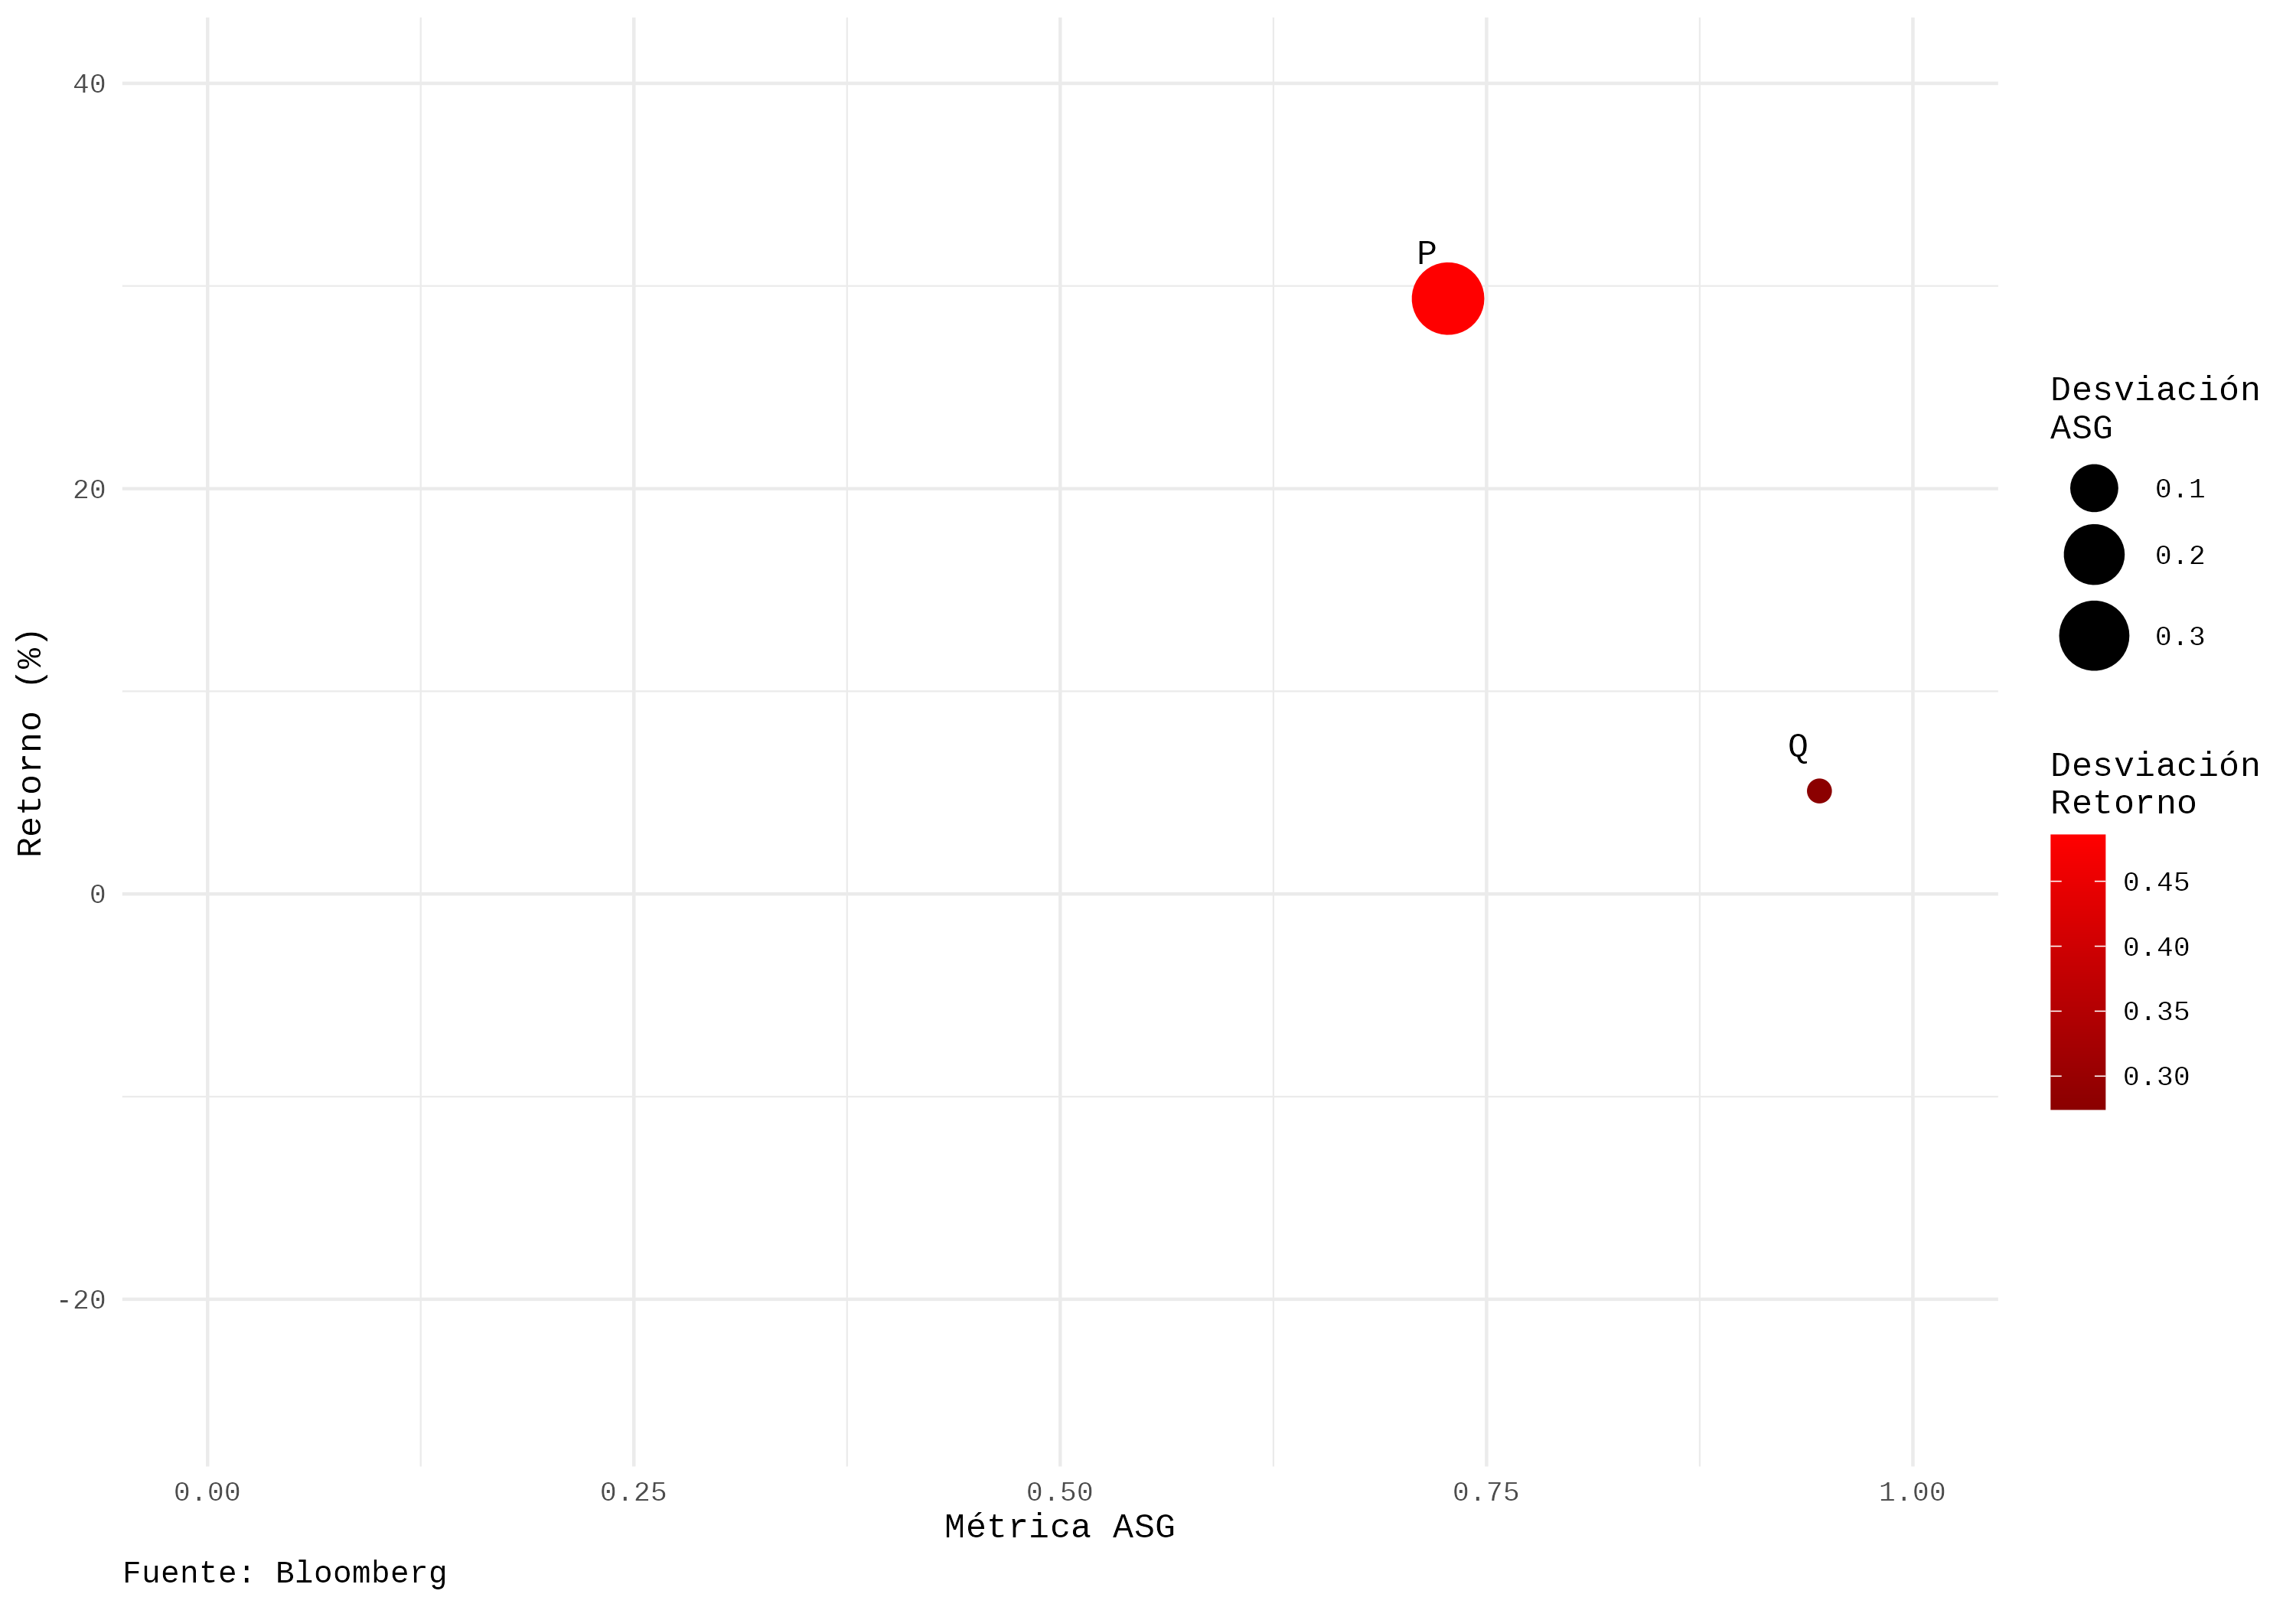
\includegraphics[width=0.65\linewidth]{plot_4YTD.png}
        \caption{Ejemplo de Ensayo}
    \end{figure}
\end{frame}


\begin{frame}
    \frametitle{Metodología y Herramientas Utilizadas}
    \begin{itemize}
        \item Esta metodología ayudó a entender cómo los diferentes perfiles demográficos y niveles de experiencia financiera reaccionan ante las opciones de inversión presentadas.
    \end{itemize}
    \begin{figure}
        \centering
        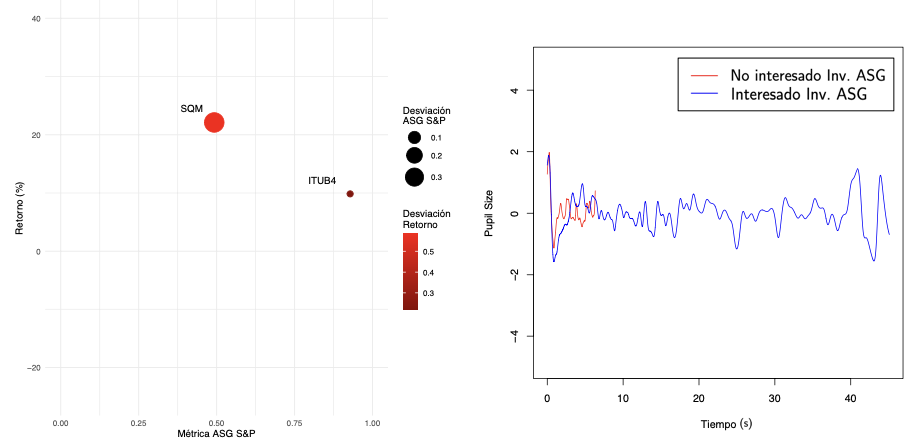
\includegraphics[width=0.7\linewidth]{Latex/defensa/perfiles_resultados.png}
        \caption{Interés en inversiones ASG vs tiempo de respuesta}

    \end{figure}
\end{frame}

\subsection{Resultados}
\begin{frame}
    \frametitle{Análisis de Decisiones}
    \begin{itemize}
        \item \textbf{Preferencias de Inversión:} Los participantes, cuando los retornos financieros eran comparables, en general eligieron el activo con mayor puntuación ASG.
    \end{itemize}
    \begin{figure}
        \centering
        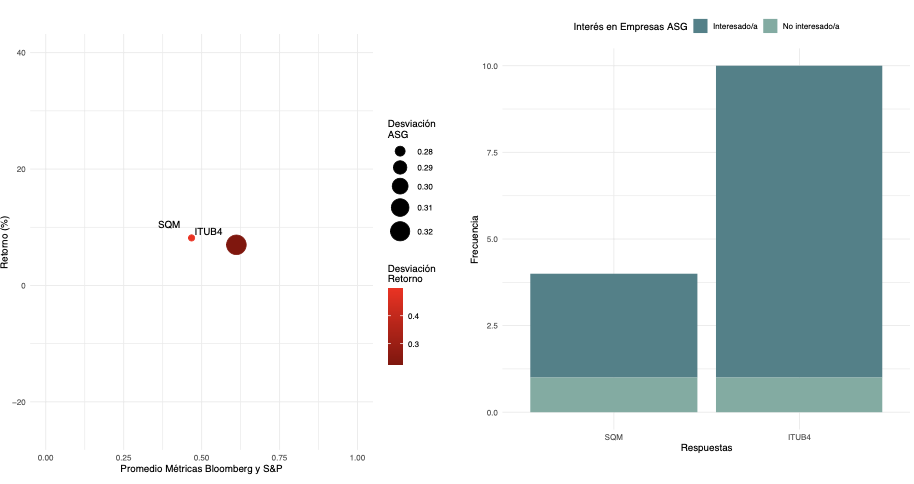
\includegraphics[width=0.7\linewidth]{Latex/defensa/eleccion.png}
        \caption{Elecciones con retornos comparables}
    \end{figure}
\end{frame}

\begin{frame}
    \frametitle{Análisis de Decisiones}
    \begin{itemize}
        
        \item \textbf{Impacto de la Información ASG:} La manera en que se presenta la información ASG cambia las decisiones que toman algunos participantes, lo que significa que la manera de mostrar los datos influye en las decisiones de inversión. Dos de tres individuos no fueron consistentes con lo respondido en la valoración contingente comparado con el ensayo respectivo.
    \end{itemize}
\end{frame}





\section{Conclusiones}

\subsection{Conclusiones Generales}
\begin{frame}
    \frametitle{Conclusiones}
    \begin{itemize}
        \item \textbf{(C1) Importancia de la Información ASG:} Los inversionistas consideran prácticas ASG como un beneficio en sus inversiones. Sin embargo, cada uno los considera de distinta manera dependiendo de sus creencias y valores.
        
    \end{itemize}
    \begin{figure}
        \centering
        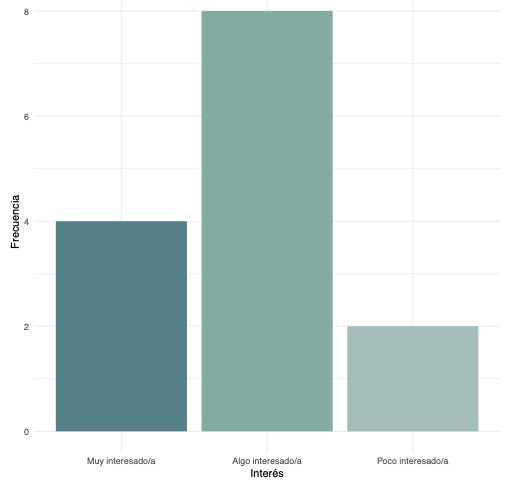
\includegraphics[width=0.4\linewidth]{Latex/defensa/interes_inv_asg.png}
        \caption{Interés en invertir en empresas con practicas ASG}
    \end{figure}
\end{frame}

\begin{frame}
    \frametitle{Conclusiones}
    \begin{itemize}
        
        \item (C2) A través de la metodología de Valoración Contingente, se observó que los participantes no están dispuestos a asumir un costo mayor al 10\% de rentabilidad monetaria a cambio de aumentar en 44\% el retorno ASG, lo que se traduce en que el retorno monetario es el factor más influyente en la toma de decisión en el experimento. 
    \end{itemize}
\end{frame}


\subsection{Trabajos Futuros}
\begin{frame}
    \frametitle{Futuras Mejoras}
    \begin{itemize}
        \item \textbf{Ampliar la Muestra:} Futuras investigaciones podrían beneficiarse de una muestra más grande y diversa para generalizar los resultados a una población más amplia. 
        
        \item \textbf{Presentar Información de Otra Manera:} Presentar la información de manera progresiva puede resultar en distintos estímulos, lo que se puede observar en la dilatación dependiendo de la atención que el individuo le tome a esa nueva información. Además, presentar la información de manera más clara e intuitiva. 
        
        \item \textbf{Limitar el tiempo:} Definir un tiempo fijo en el que se presenta la información permite hacer la comparación de datos entre individuos más fácil.
    \end{itemize}
\end{frame}

\begin{frame}
\centering
    \huge \textbf{¡Gracias!}
\end{frame}



%----------------------------------------------------------------------------------------
%   ANEXOS - GRÁFICAS
%----------------------------------------------------------------------------------------
\section{Anexos}
\subsection{Gráficas del Estudio}

% Ejemplo de diapositiva con dos gráficas
\begin{frame}
    \frametitle{Anexos - Gráficas}

    \begin{minipage}{0.52\textwidth}
    \begin{figure}
        \centering
        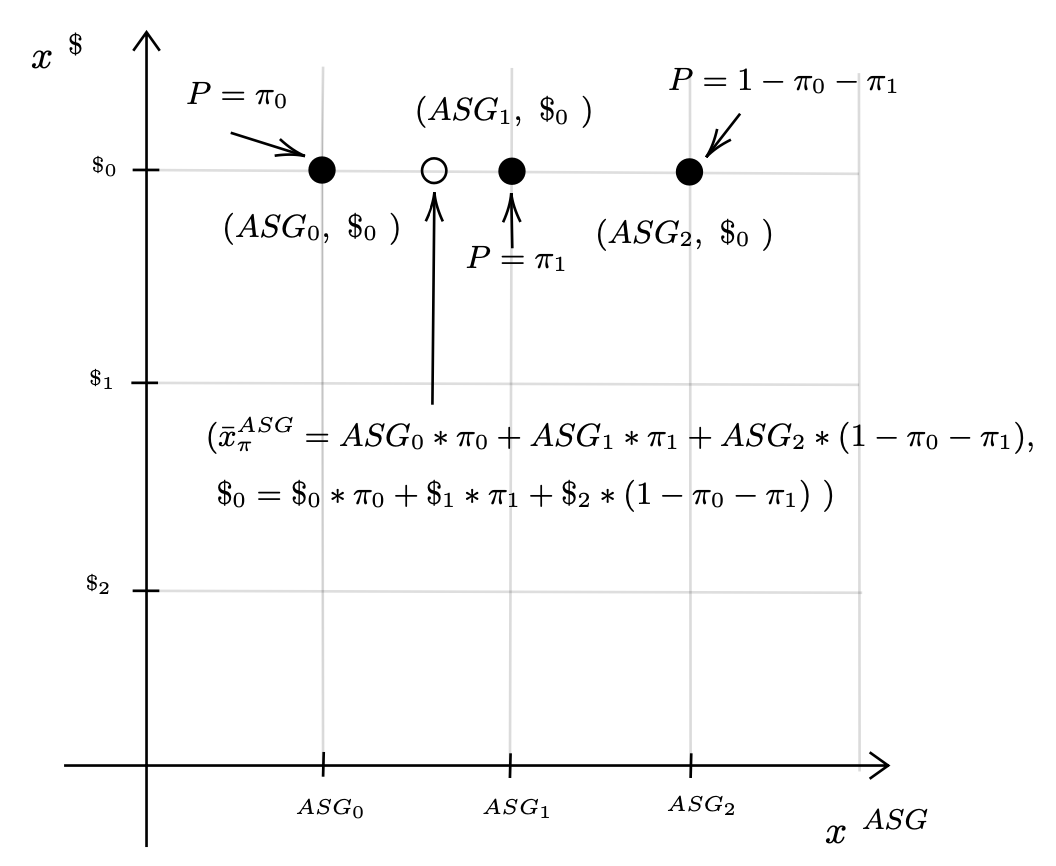
\includegraphics[width=\textwidth]{EjemploActivoJ.png}
        \caption{Ejemplo Ponderación}
    \end{figure}
    \end{minipage}
    \hfill
    \begin{minipage}{0.45\textwidth}
    \begin{figure}
        \centering
        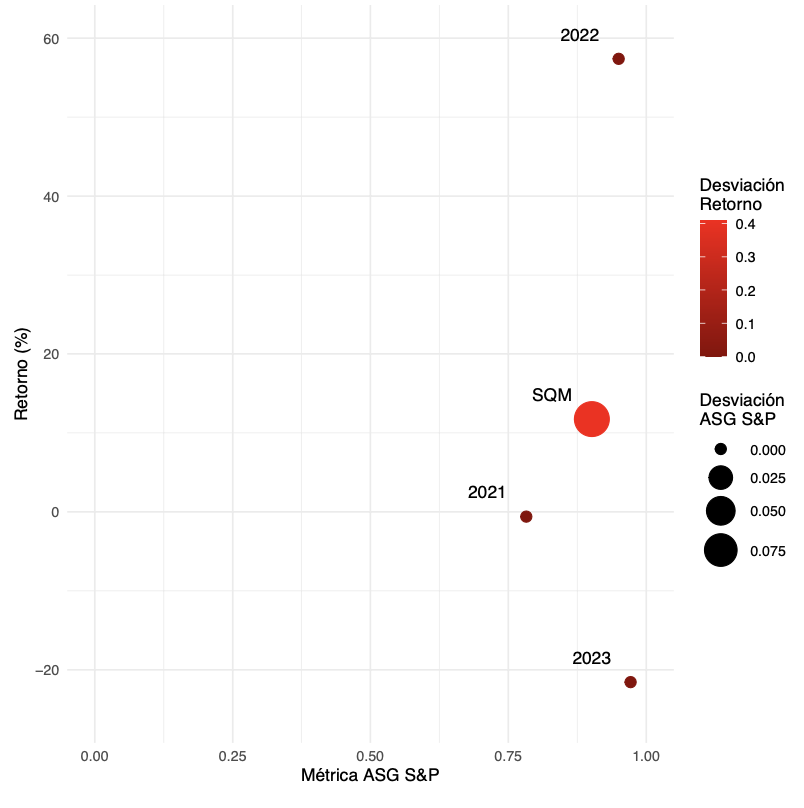
\includegraphics[width=\textwidth]{EjemploPonderacionSQM.png}
        \caption{Ejemplo Ponderación SQM}
    \end{figure}
    \end{minipage}
\end{frame}



% Ejemplo de otra diapositiva con dos gráficas
\begin{frame}
    \frametitle{Anexos - Tabla de Datos}
    \begin{table}
        \caption{Datos por periodos de tiempo}
        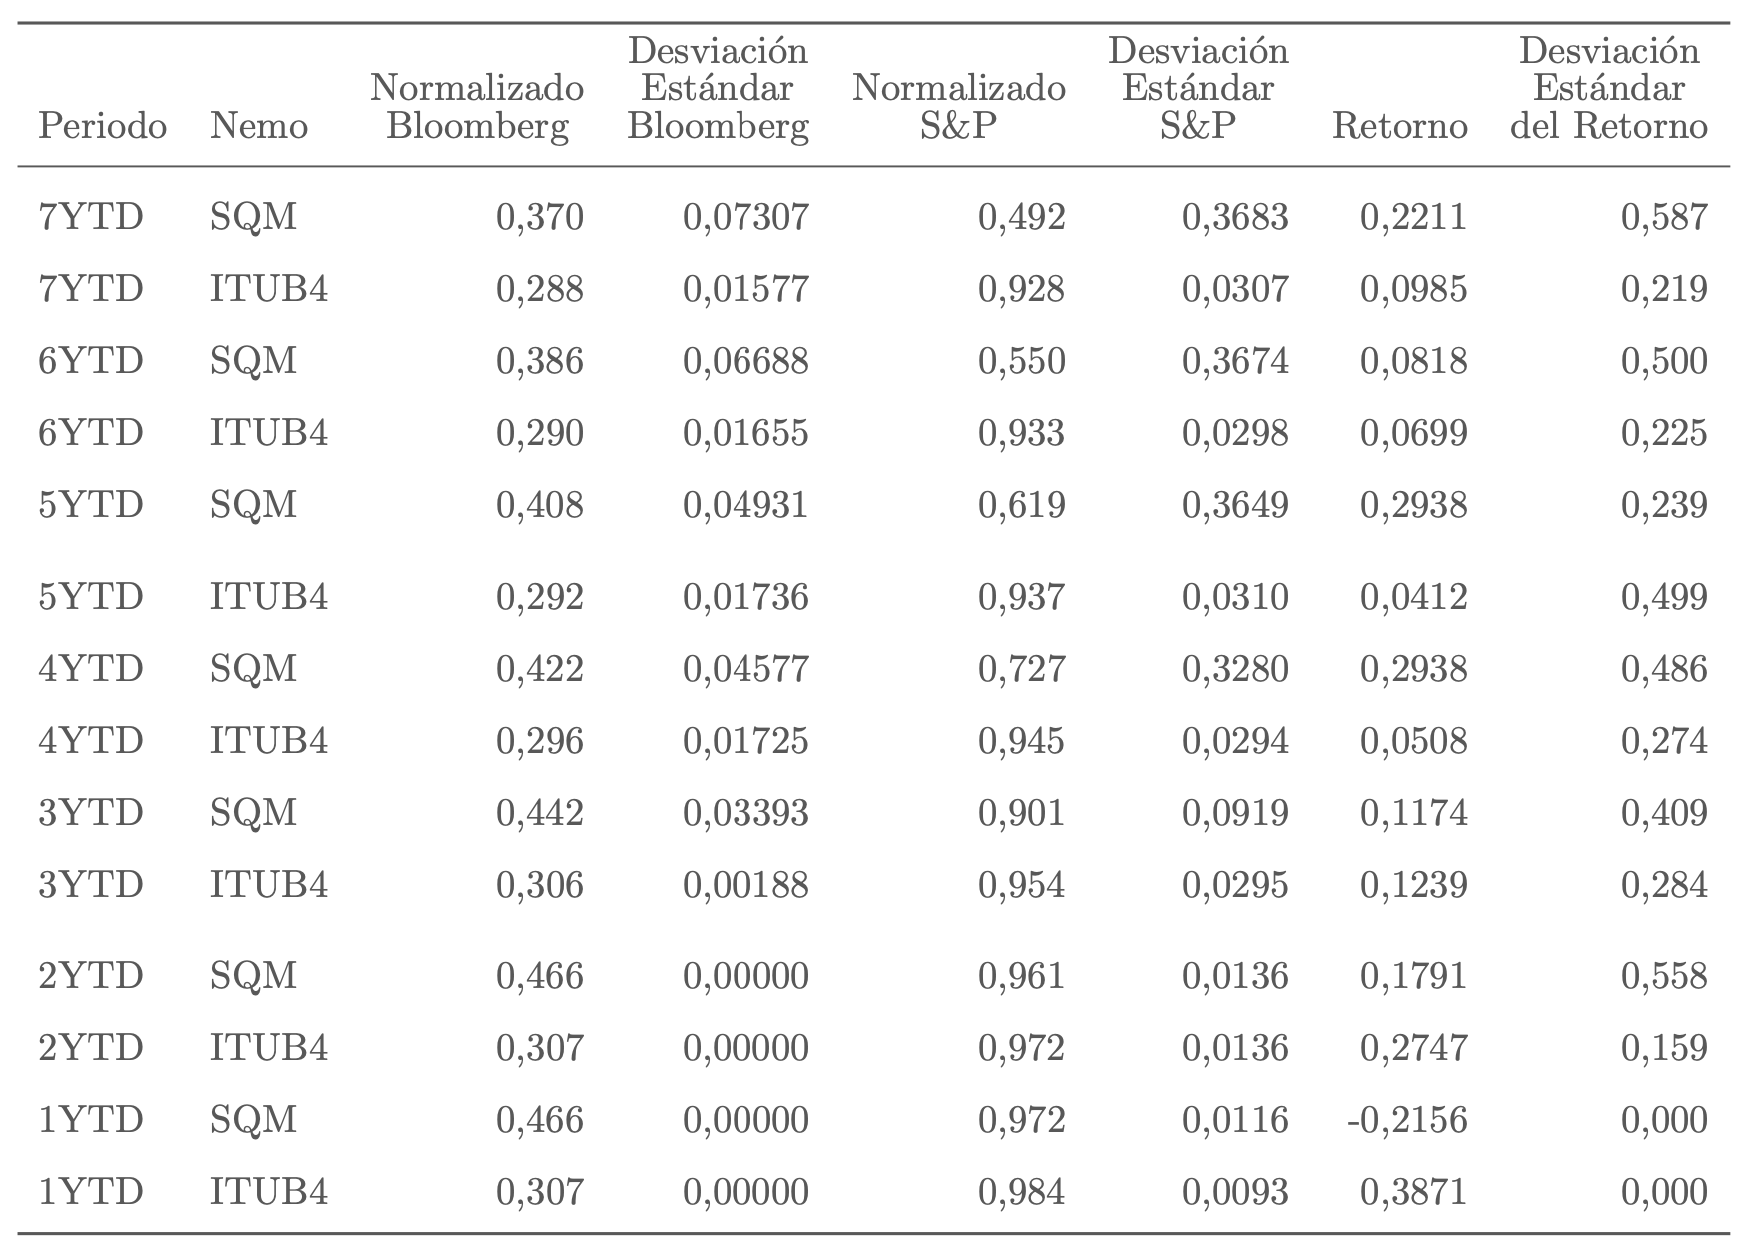
\includegraphics[width=0.8\textwidth]{Datos.png}
    \end{table}
\end{frame}

\begin{frame}
    \frametitle{Anexos - Valorización Contingente}
    \begin{figure}
        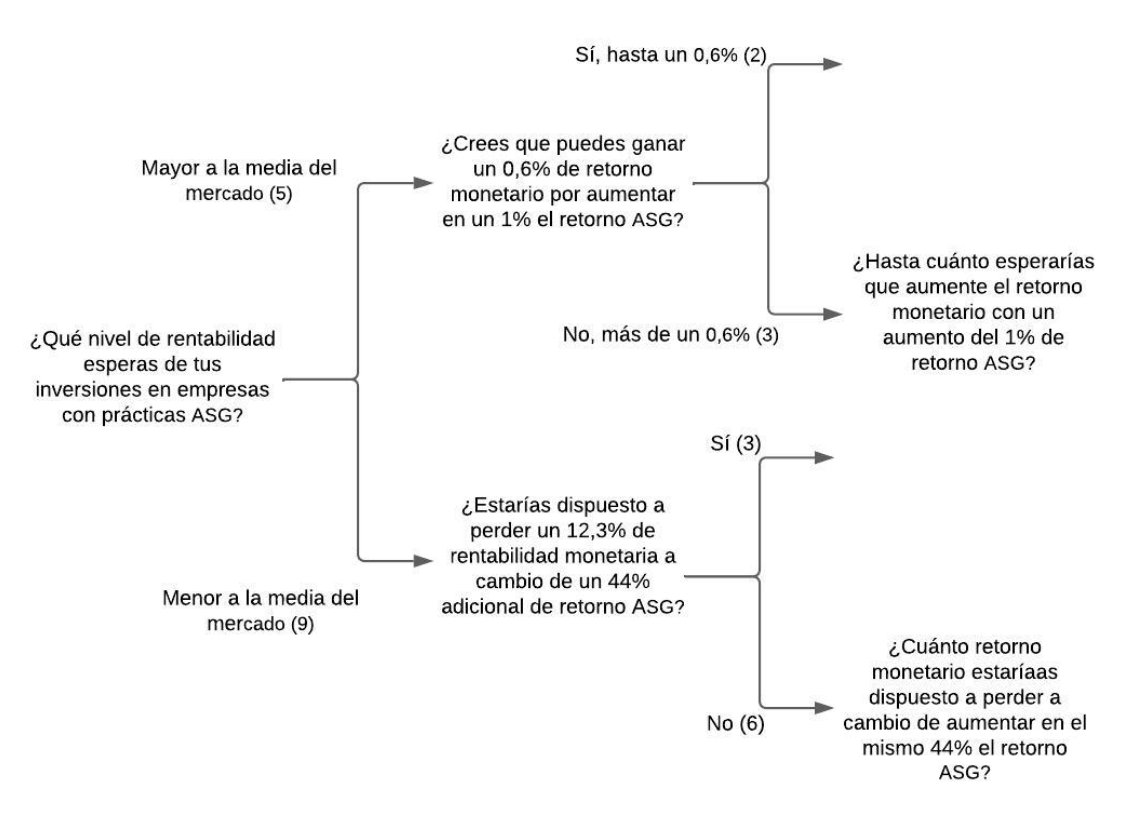
\includegraphics[width=0.8\textwidth]{DiagramaValorizacionContingente.png}
        \caption{Diagrama Valorización Contingente}
    \end{figure}
\end{frame}

\begin{frame}
    \frametitle{Anexos - Caso Respuesta Racional}
    \begin{figure}
        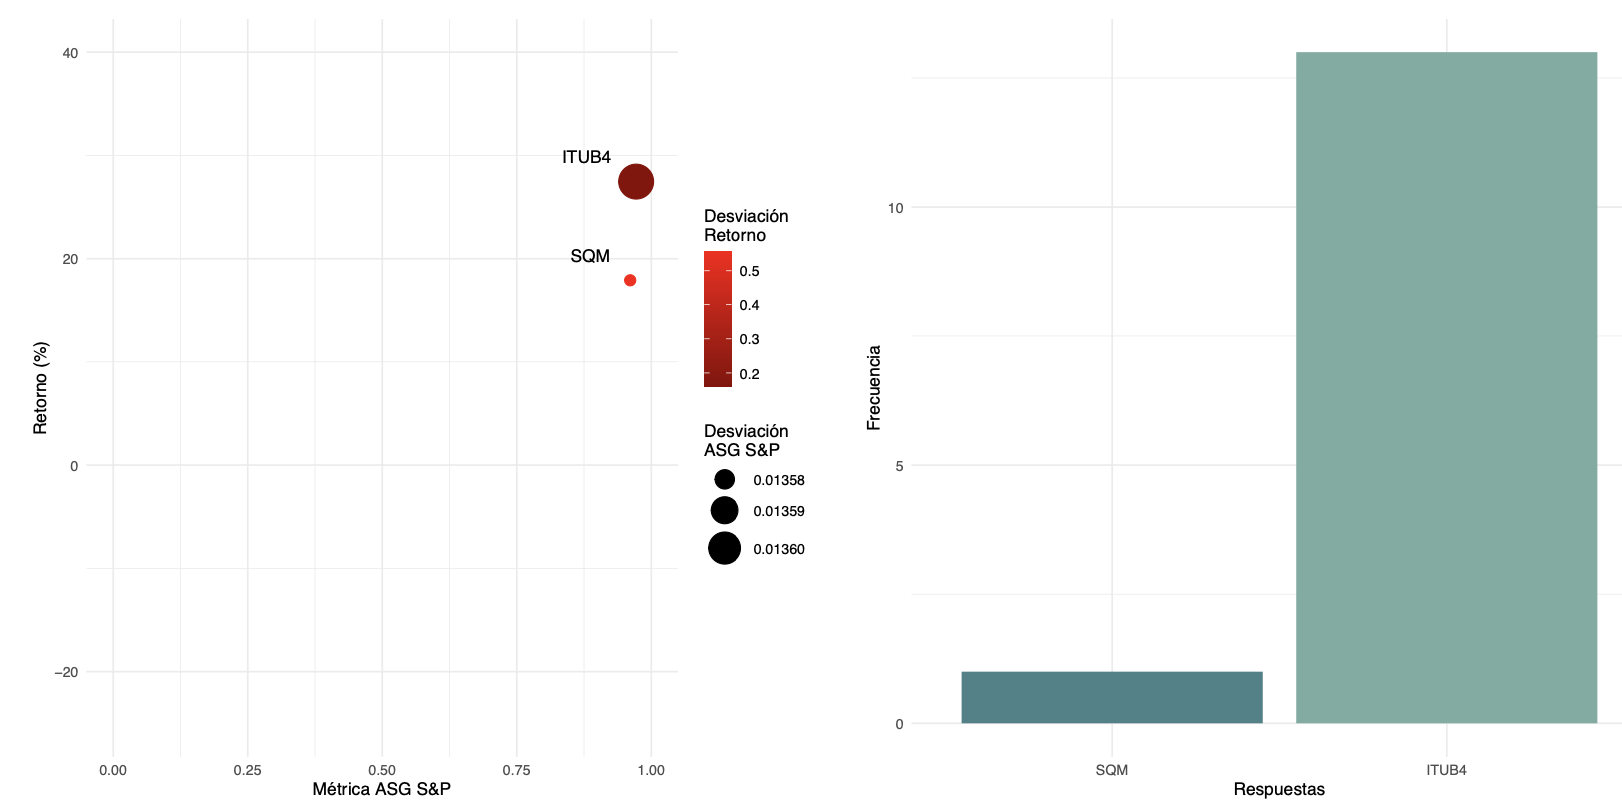
\includegraphics[width=1\textwidth]{CasoRespuestaRacional.png}
        \caption{Caso con Respuesta Racional Definida}
    \end{figure}
\end{frame}

\begin{frame}
    \frametitle{Anexos - Ejemplo de Caso con Decisión}
    \begin{figure}
        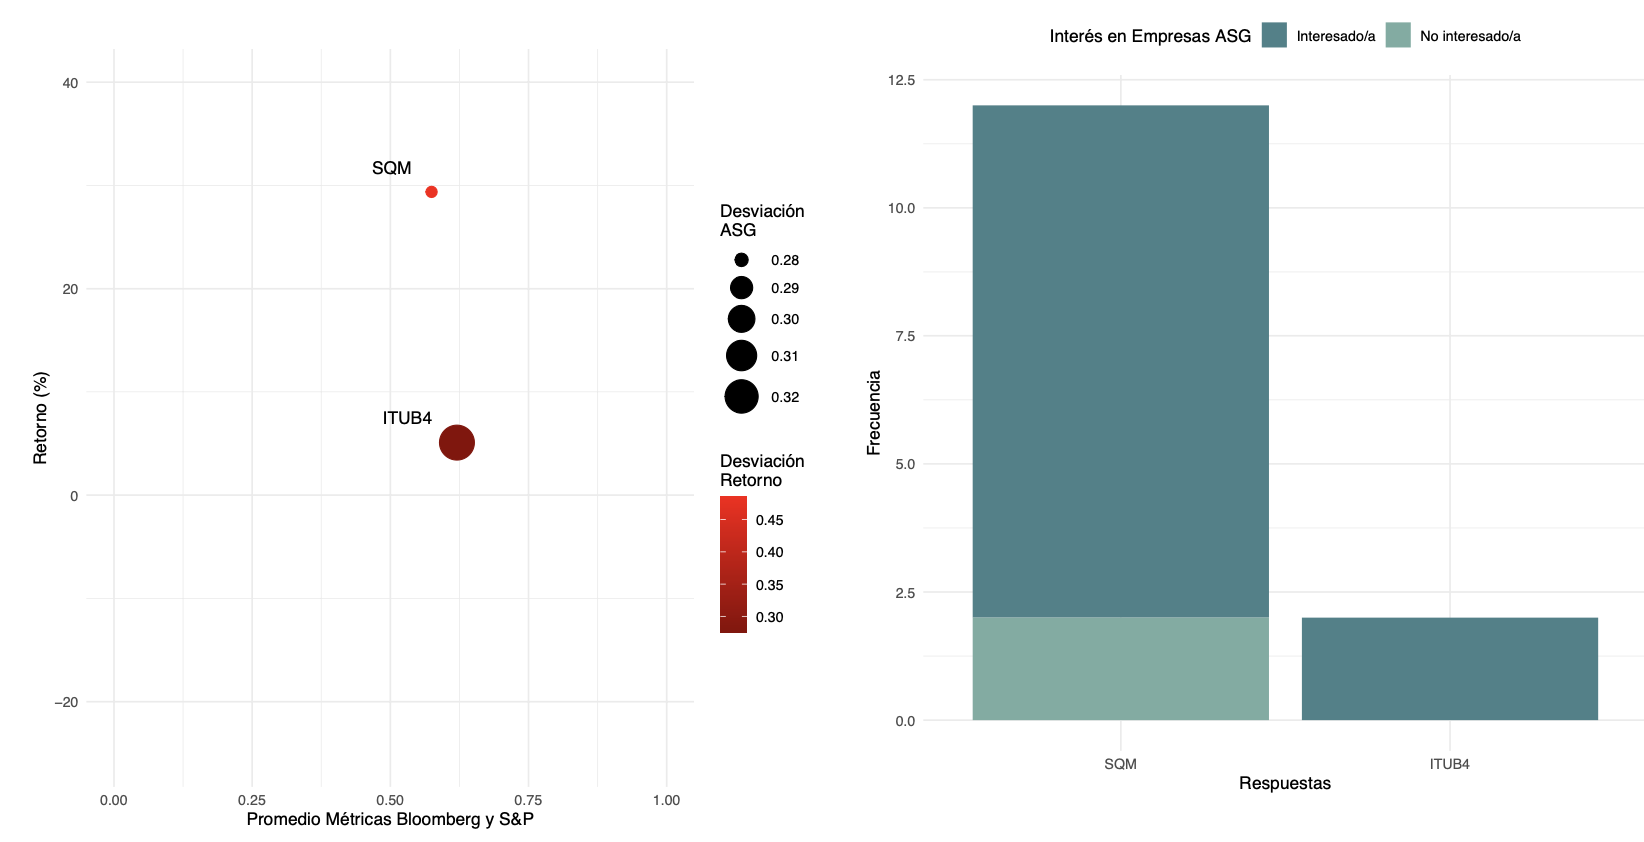
\includegraphics[width=1\textwidth]{Decision.png}
        \caption{Gráfica y Respuestas a 4 años (S\&P y Bloomberg)}
    \end{figure}
\end{frame}

\begin{frame}
    \frametitle{Anexos - Datos de Pupila}
    \begin{figure}
        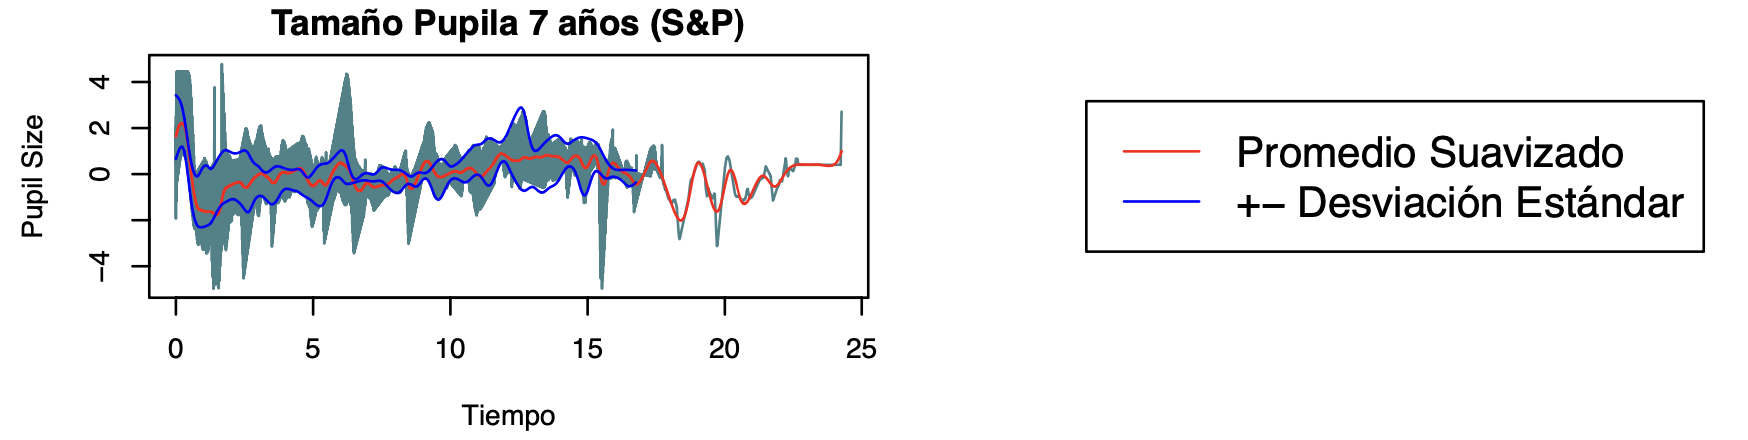
\includegraphics[width=1\textwidth]{DatosPupilares.png}
        \caption{Ejemplo Datos de Pupila}
    \end{figure}
\end{frame}

\begin{frame}
    \frametitle{Anexos - Datos de Pupila Comparado con CRT}
    \begin{figure}
        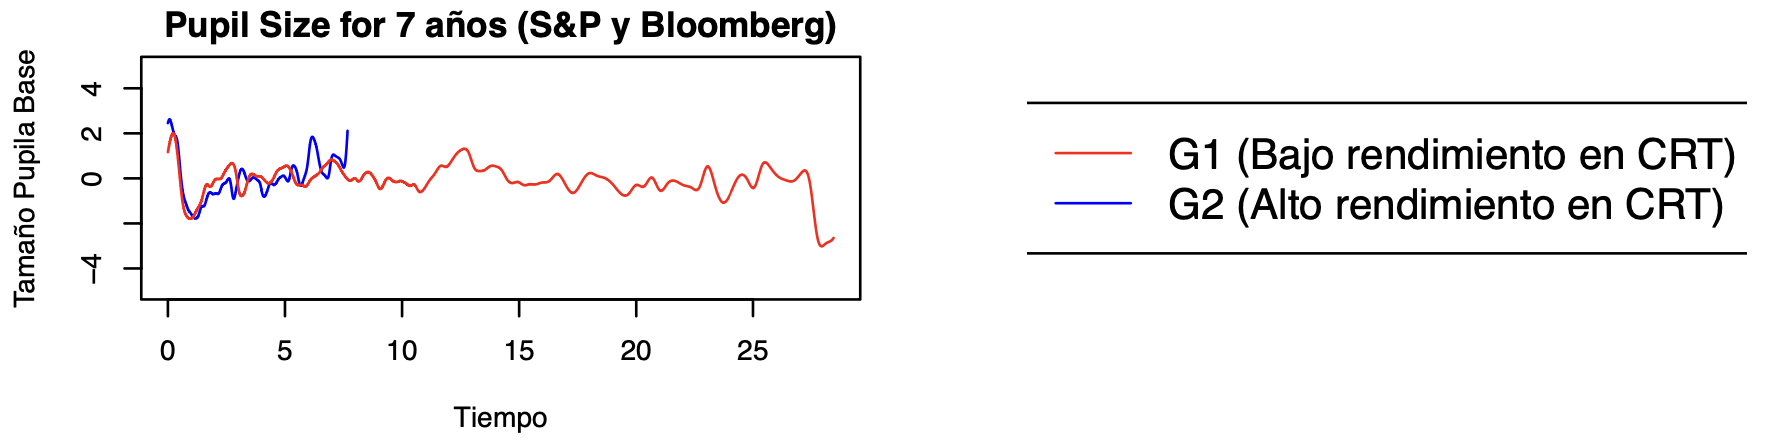
\includegraphics[width=1\textwidth]{DatosPupilaCRT.png}
        \caption{Datos de Pupila Comparados a CRT}
    \end{figure}
\end{frame}

\begin{frame}
    \frametitle{Anexos - Retorno SQM 2022}
    \begin{figure}
        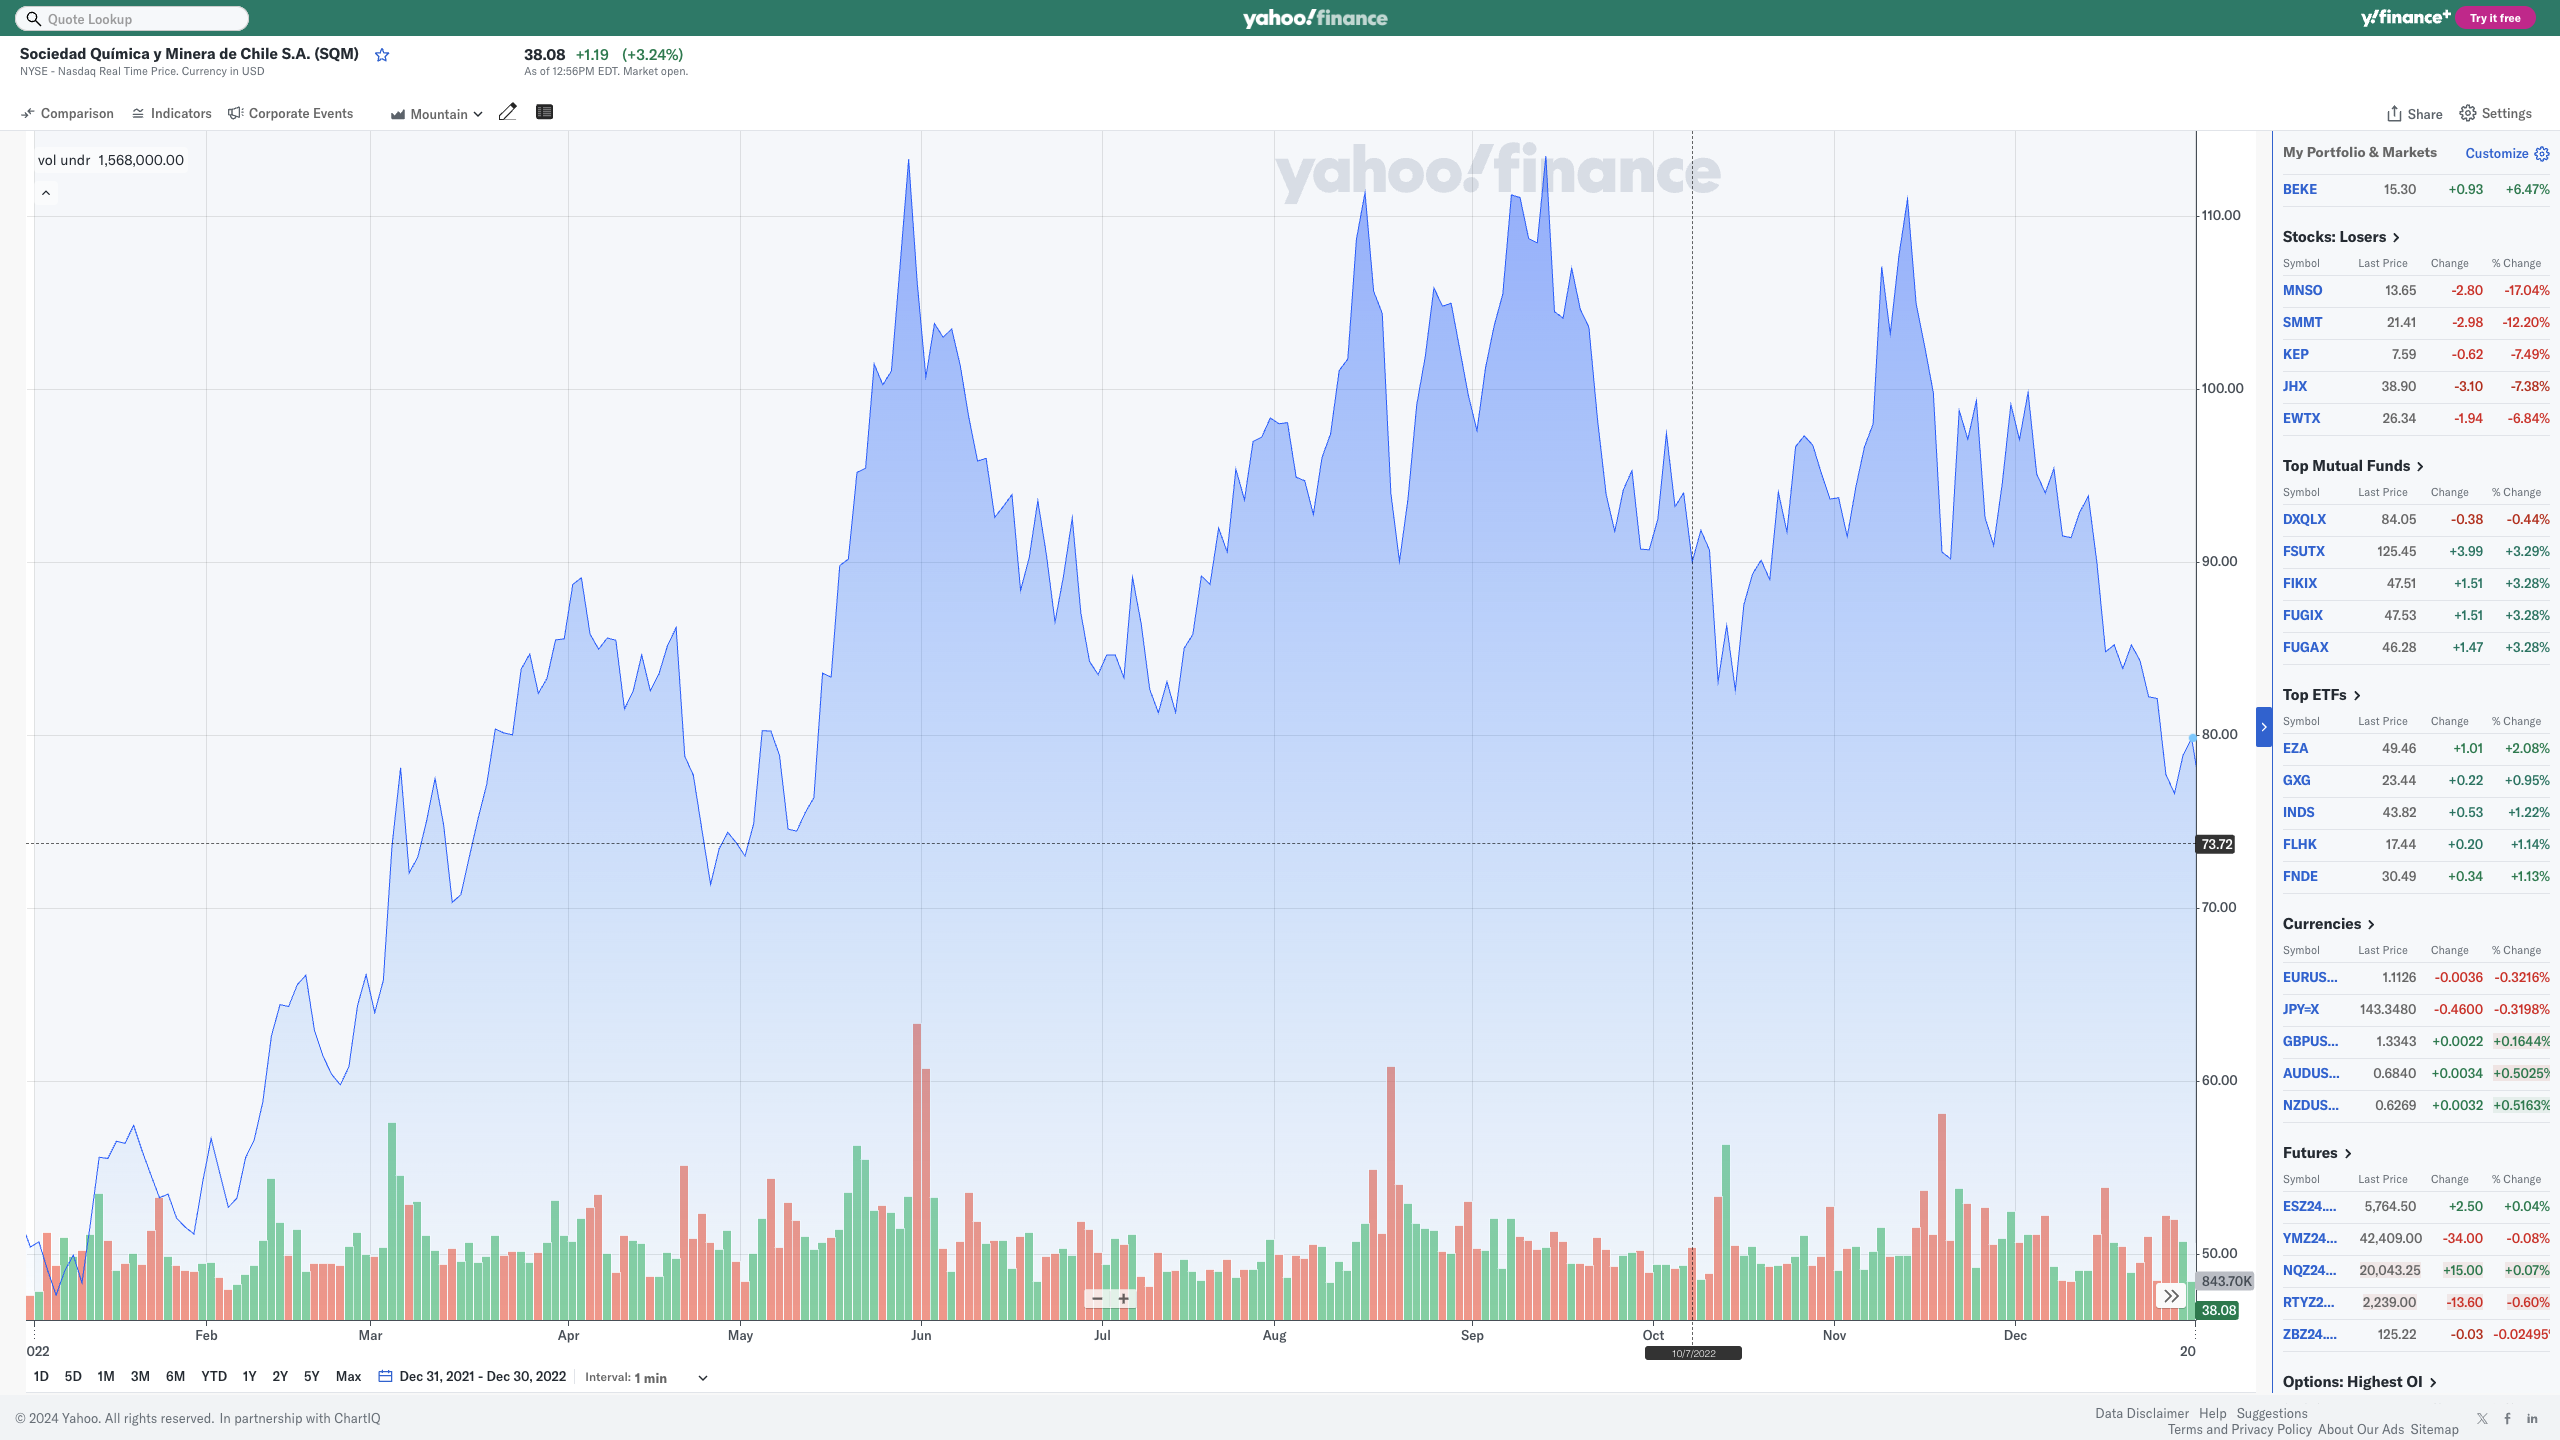
\includegraphics[width=1\textwidth]{retorno2022SQM.png}
        \caption{Retorno SQM año 2022}
    \end{figure}
\end{frame}

\begin{frame}
    \frametitle{Diseño y Configuración del Experimento}
    \begin{itemize}
        \item Los participantes firmaron un consentimiento informado antes de comenzar el experimento, documento revisado junto al Comité de Ética de la Universidad de Los Andes.
        \item Utilización del programa OpenSesame para administrar el experimento y recoger datos de seguimiento ocular en tiempo real mediante el uso de librería integradas.
    \end{itemize}
    \begin{figure}
            \centering
            
\includegraphics[width=0.8\linewidth]{Latex/defensa/logo_opensesame.png}
        \end{figure}
\end{frame}

\bibliography{Latex/docs/references}

\end{document}

